\chapter{The better web application architecture, Flux or MVC?}
\label{cha:fluxreduxmvc}

Variants of the programming paradigm, Model-View-Controller (MVC), are the most common architectural choices to program user interface applications in the web. Facebook introduced a supposedly new programming paradigm named Flux. This chapter will not only introduce the reader to Flux, but also critically compare it to the MVC pattern. The comparison will reveal advantages and disadvantages of programming a web application with either of the previously mentioned paradigms.

%Reading this chapter will also show the reader how to design a React application, how to make it scalable and extensible using Redux, an implementation of Flux. 

\section{Introduction to Flux}

Flux was introduced by Facebook in mid 2014 and on the official website \cite{FacebookInc.2014} the paradigm is described as an application architecture that is used by Facebook to build client-side, single-paged applications. It is clearly stated, that Flux is a programming pattern and not a framework. The source also claims that Flux can easily be implemented in conjunction with Facebook's ReactJS framework because of React's composable view components. In fact, Flux was designed to work well with Facebook's framework ReactJS to increase productivity and the scalability of the application using the framework with the Flux architecture. There will be an in-depth explanation of ReactJS in the Chapter \ref{cha:ReactJS} of this bachelor's thesis.

\subsection{Structure and Dataflow}

The most important aspect of Flux is dataflow. Facebook's statement to the mindset of a programmer using Flux \cite[structure-and-data-flow]{FacebookInc.2014} is that the unidirectional dataflow is central to the Flux pattern and should be the primary mental model for the programmer. 

% debuggability and better overview over code? add smth like that?

The Flux application architecture consists of 3 main components: The Dispatcher, the Store and the View as it can be observed in the Figure \ref{fig:FluxArchitecture}. Unidirectional dataflow is achieved by only accessing application state via the Dispatcher. The Dispatcher can only manipulate the Store's data by dispatching so-called Actions that reduce the application state to the desired state. Reducing the state means that it is manipulated from the current state to the a new state. This so-called reducer functions are pure functions that can be tested very well. The Store then automatically and implicitly updates the View. 

% ReactJS is perfect for the Flux architecture because it listens for changed component properties and updates itself accordingly. The Store's data is initially passed to the root component of the ReactJS component tree as a property. If data changes, the React root component updates the whole component tree by implicitly looking for changes in the application state by observing the root property. 

\begin{figure}
  \centering
  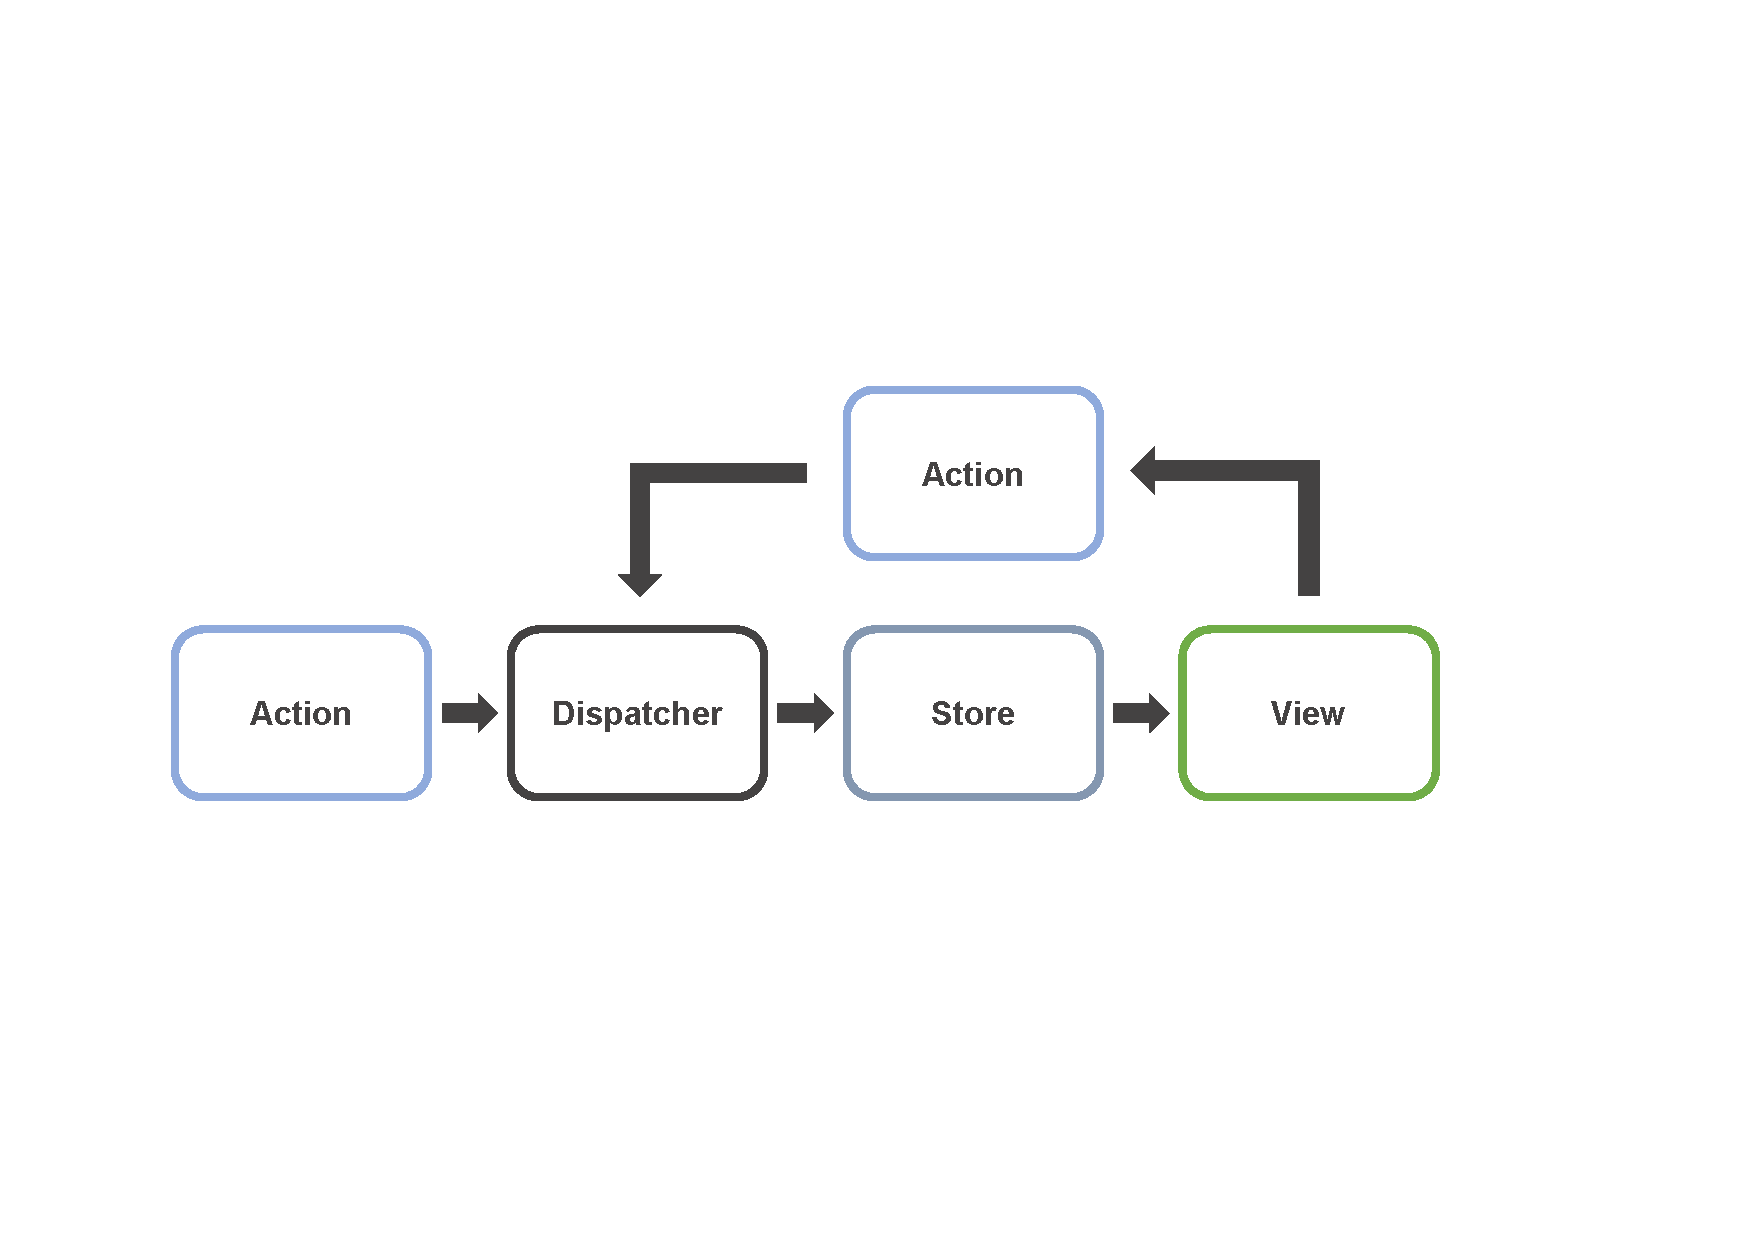
\includegraphics[scale=.6, trim= 2.5cm 6cm 4cm 6cm, clip]{002Flux.pdf}
  \caption{Flux application architecture \cite[as in][structure-and-data-flow]{FacebookInc.2014}}
  \label{fig:FluxArchitecture}
\end{figure}

After understanding the fundamental concept of Flux, it should also be of interest for the programmer to fully understand the function of each component of the paradigm. It is important to know about the whole concept and all of its components to further being able to understand implementations of Flux or Flux frameworks.

\subsection{Dispatcher}

In the documentation \cite[a-single-dispatcher]{FacebookInc.2014}, a Dispatcher is specified as a "central hub that manages all dataflow in a Flux application". A very important fact stated in \cite[actions]{FacebookInc.2014} is, that a Dispatcher exposes a method, which can be passed an Action. If provided an Action via that method, the Dispatcher then dispatches that Action to all Stores, triggering an update only on Stores that can react to the dispatched Action. One of the biggest advantages is that many Stores can react to the same Action, which makes the application highly scalable and extensible.  

The dispatcher can also explicitly handle more than one Store by handling their registered callbacks in a specified order, if that behavior is desired by the web application programmer.

When the application grows, there can be more than one Action set. The programmer should logically divide all available actions into different files to keep the application organized. This does not change the fact that all actions are dispatched with the same Dispatcher to all registered Stores. 

\subsection{Store}
\label{ssec:fluxstore}

% revisit citations

As it can be read in \cite[structure-and-data-flow, Stores]{FacebookInc.2014}, a Store contains an application-specific state and data, as well as data manipulation logic. Every Store has to be registered to the Dispatcher by registering a callback. 

Registered callbacks can be used to handle asynchronous data change events in the Store. The Dispatcher uses the Store's callbacks to determine when a data transaction or manipulation has finished in order to being able to dispatch a new action. Registered callbacks are also used to dispatch actions in a specific order to more than one Store.

As mentioned above, Stores also contain data manipulation logic. The way Stores work in conjunction with Dispatchers is that the Dispatcher dispatches one Action to all registered Stores. Each Store can react to that dispatched Action with its own internal data reducing functions.

\subsection{View}

The View component is responsible for correctly displaying any state of provided data as described in \cite[views-and-controller-views]{FacebookInc.2014}. To achieve that, so called Controller-Views can handle data from any Store and also pass it down to any nested component in the view hierarchy.

Controller-Views react to Store update events and can update whole child component trees by updating their own internal state. By reacting to any data changing event, the Controller-View triggers an update for its child component tree. Each child component can then process the passed data from the parent component, only processing component relevant data. The programmer could even decide to pass a whole Store's data to a Controller-View.

Every important section of a web application should be considered as a Controller-View. In ReactJS it is very easy to determine what components are Controller-Views. As explained in Chapter \ref{cha:ReactJS}, ReactJS Containers are the so called \enquote{smart} components and could be considered as Controller-Views in the Flux pattern. Again, the Flux pattern works exceptionally well with ReactJS, as ReactJS components automatically trigger a render refresh if component properties change. With Flux the programmer only has to introduce a root component bound to the Stores data in order to automatically re-render the application if the Store's data has changed.

\subsection{Action} \label{ssec:fluxaction}

The creation of Actions is handled by action creator methods worked out in \cite[structure-and-data-flow, actions]{FacebookInc.2014}. An Action can be created by a user interaction through an event handler of the corresponding view, through an initialization of a component or even through the server sending an error code for example. As explained before, the Action is then dispatched to the Stores to be handled and to manipulate the Stores to the desired state.

If the application needs to communicate with some kind of API or execute any asynchronous operation it is usually handled inside the action-creator methods. These asynchronous operations are performed and data that might result from those API-calls is then bundled into the Action and dispatched via the Dispatcher.

\section{Overview of MVC}

%% history explanation
%% fowler sehr interessant mit view und controller observed model
%% problem -> javascript nicht interchangable components, keine interfaces, patterns? flux hoax? omg :O

As mentioned before, MVC is the most common application architecture in the web. To understand the differences between Flux and MVC, this section provides all necessary information about MVC. That information is intended to help the reader to understand the arguments of the comparison between the two paradigms in this bachelor's thesis. This paper, however, assumes that the reader has a basic understanding of the MVC architecture. Due to that assumption, the overview of each aspect of the MVC pattern is rather short and only shows how this paper is referring to each component of the architecture.

\begin{figure}
  \centering
  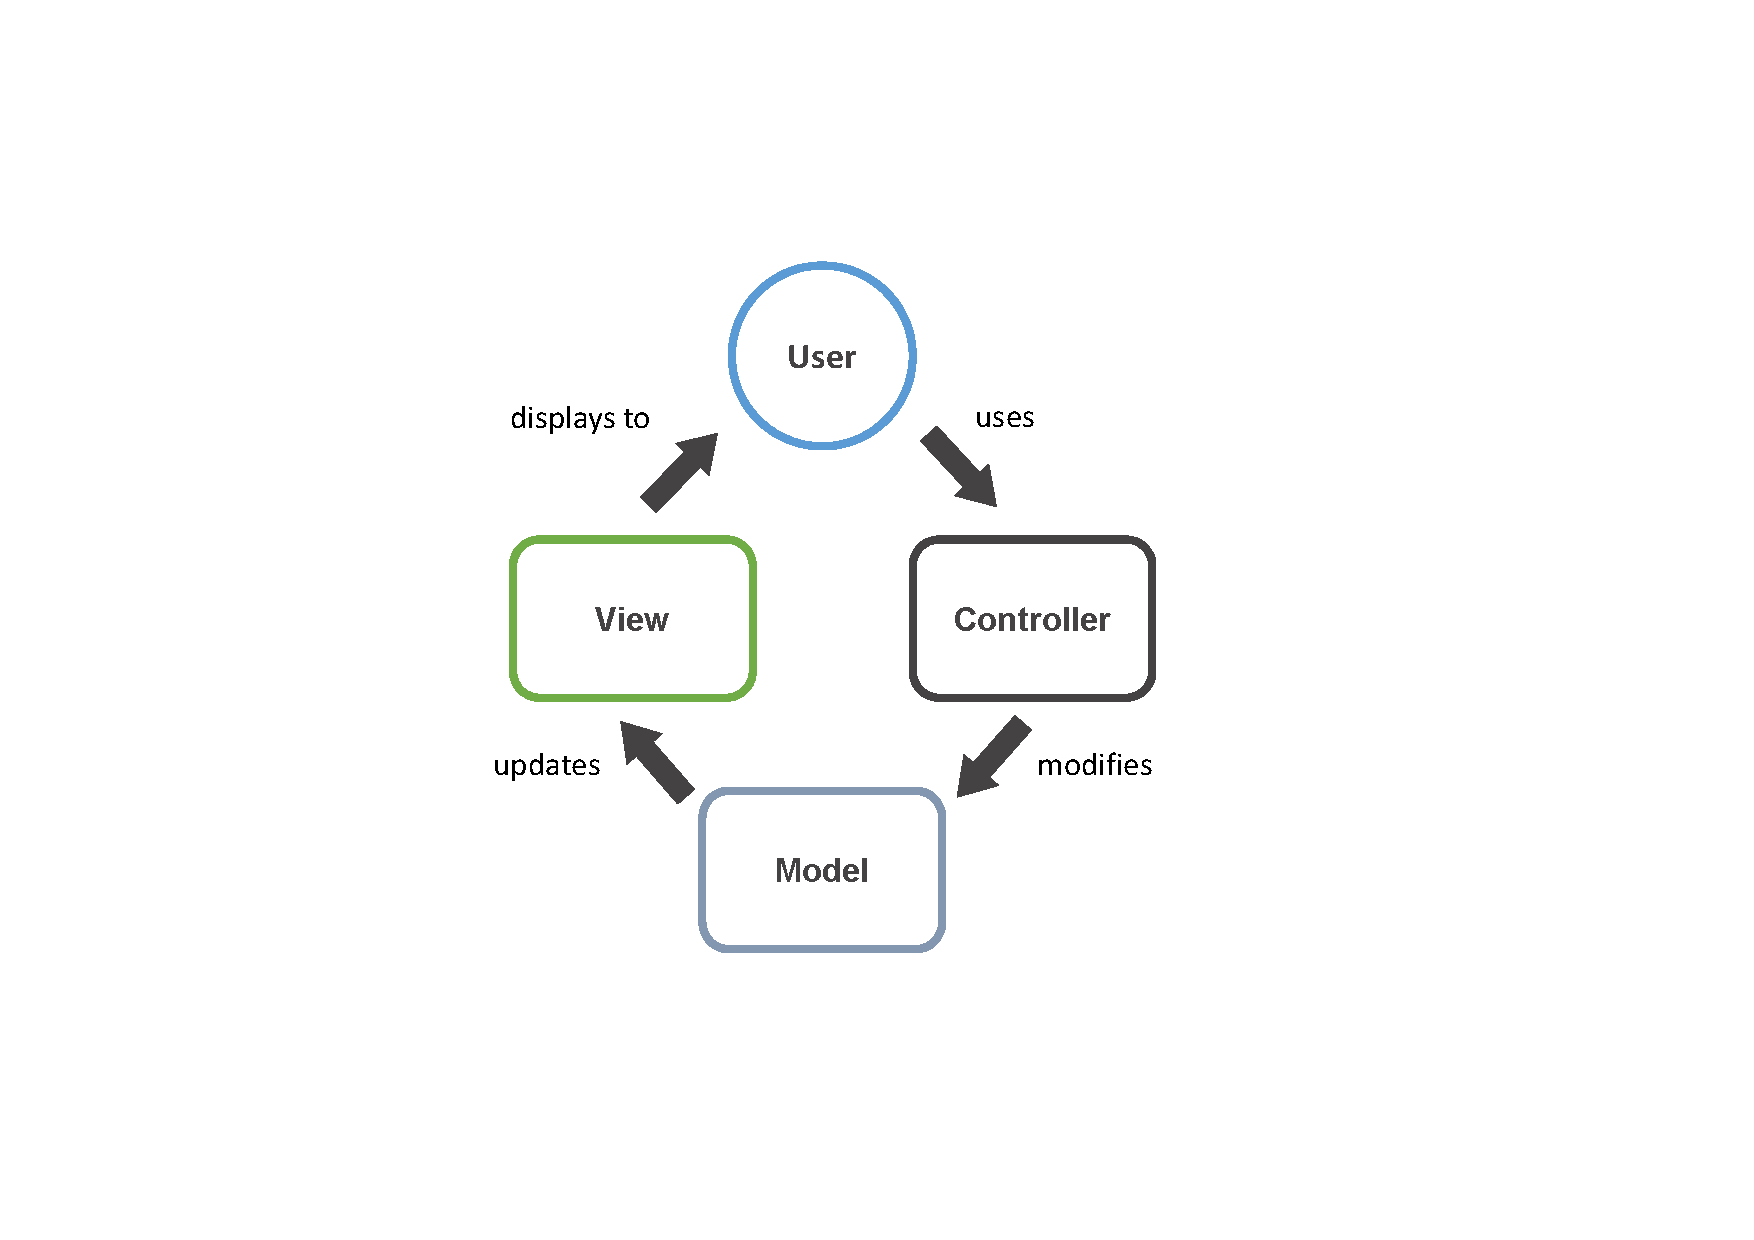
\includegraphics[scale=.7, trim= 4cm 4cm 4cm 4cm, clip]{005tradfrontendmvc.pdf}
  \caption{traditional MVC \cite[interpreted from][1.3 Traditional MVC]{stefanoborini.2014}}
  \label{fig:tradmvc}
\end{figure}

\subsection{Introduction and history}

Traditional MVC as it was initially invented and intended actually also lets data flow in one direction as shown in the Figure \ref{fig:tradmvc}. The programming pattern was invented around the year 1970 to 1980 when the concept of a user interface was not very common \cite[\#ModelViewController]{MartinFowler.2006}. The main goal was to make code of user interface applications reusable and to find a way to make UI applications scalable.

The new MVC pattern was also invented to avoid the so called "Smart-UI" anti-pattern \cite[S.11,S.13]{MattiBragge.2013}. In that paradigm there is no separation of concerns meaning that every part of the application logic is located in the interface code. It should be clear for every programmer though that such conditions should be avoided to keep the application scalable and to keep every component of the application interchangeable.

% revisit this sentence

The fact that many people are using the MVC pattern in their applications is also the reason why the pattern has many variations. There are also many different ways on how it is possible to implement an application using the programming paradigm. There are many interpretations of various aspects of the application architecture that can lead to a false understanding of MVC. This chapter will cover some of the possible misinterpretations of MVC and show how the pattern has evolved over time. It is very important get an overview to the MVC pattern in order to being able to compare it to other competing application architectures.

\begin{figure}
  \centering
  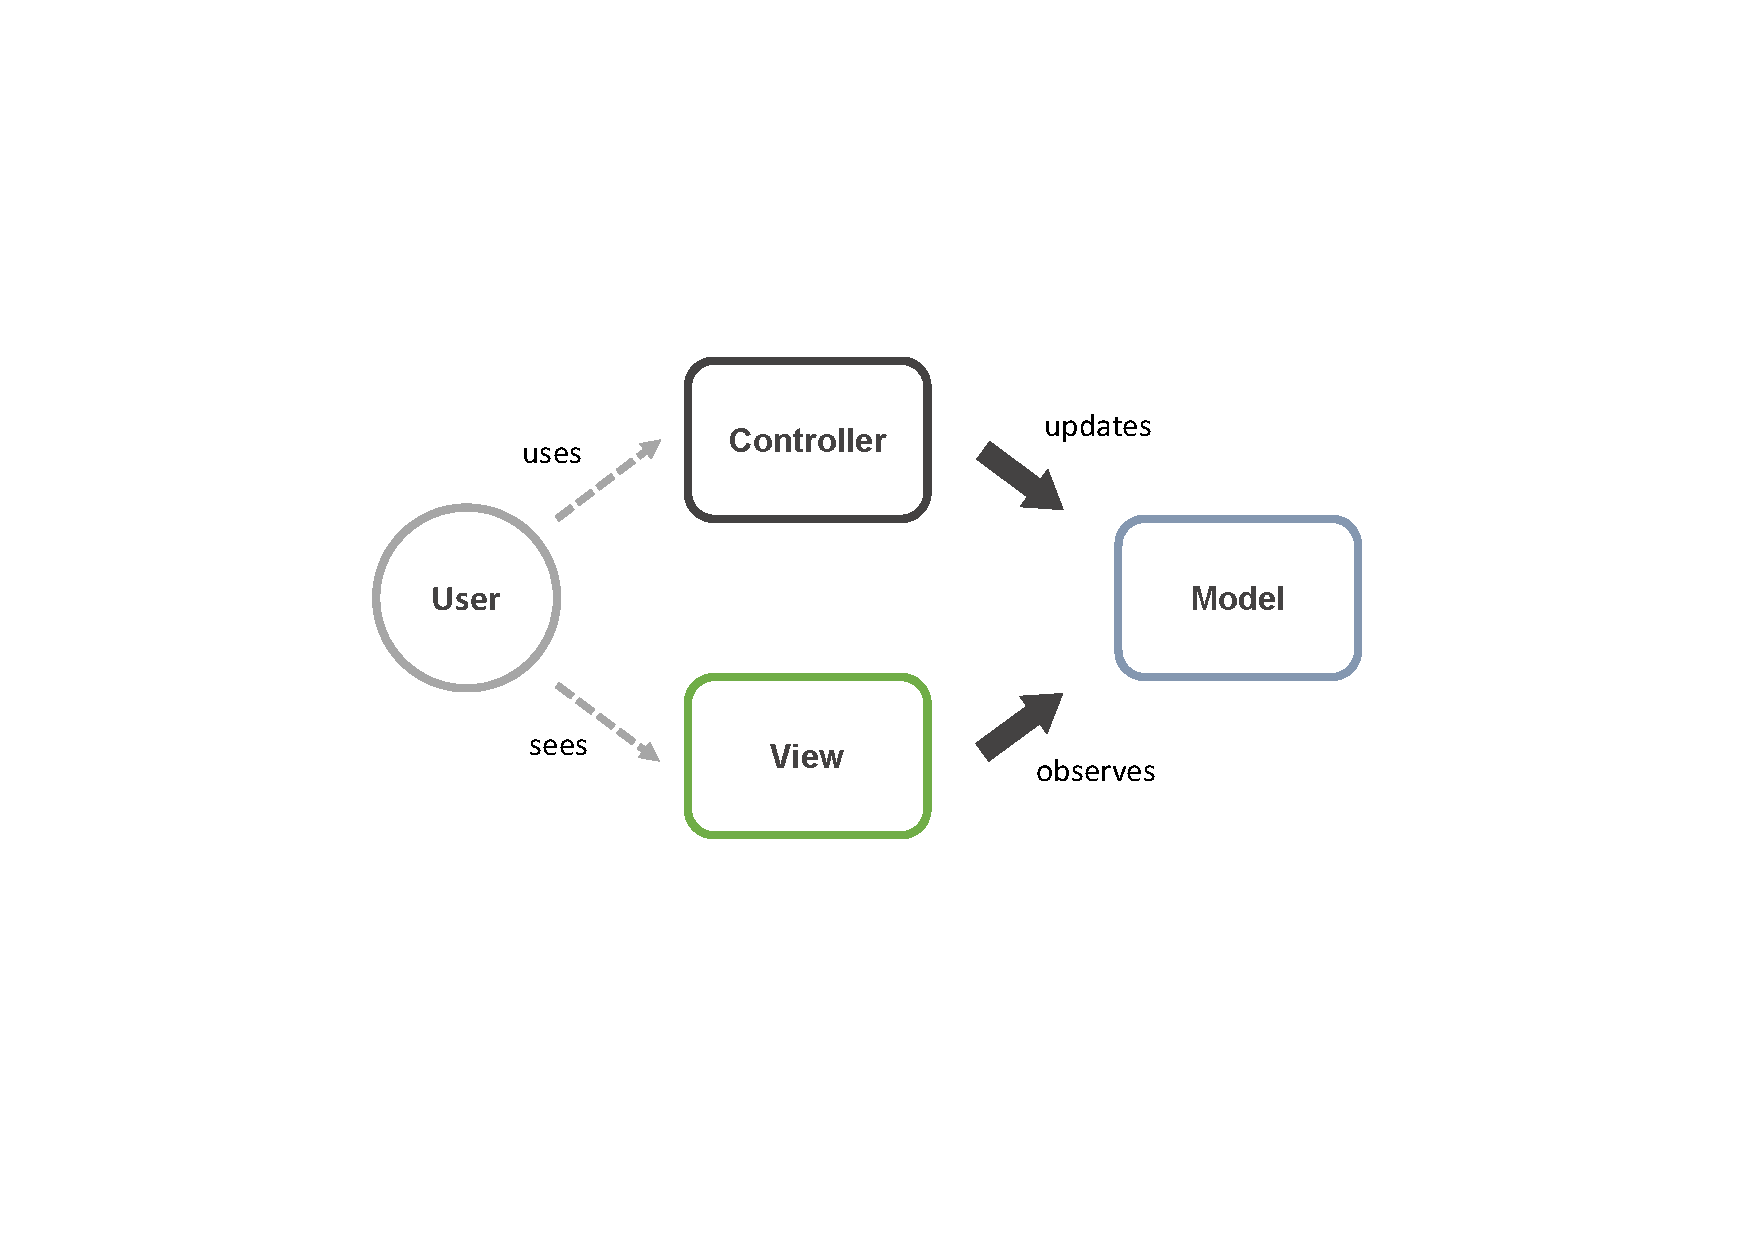
\includegraphics[scale=.7, trim= 4cm 5cm 2cm 5cm, clip]{006fowlermvc.pdf}
  \caption{another interpretation of MVC \cite[seen by][\#ModelViewController]{MartinFowler.2006}}
  \label{fig:fowlermvc}
\end{figure}

\subsection{Model}

In this paper the term "Model" is not used to represent the business logic part of the application but rather the representation of the actual application state or "real data" that is used to represent a certain state of the View (Presentation-Model). But what exactly is the Model then? In \cite[1.4.1 Model]{stefanoborini.2014} the Model is described as the component that either contains stored data or functionality to compute view-relevant data. 

The Figure \ref{fig:tradmvc} shows that the model is responsible for updating the View. Every change in the state of the model will trigger an update in the View component but not the other way around. 

According to Martin Fowler, in the Figure \ref{fig:fowlermvc}, the Model is the passive component. Fowler's MVC diagram (\ref{fig:fowlermvc}) shows the interaction arrow between Model and View in the opposite direction than the traditional MVC diagram (\ref{fig:tradmvc}). Nevertheless, this does not imply that data is flowing in the different direction---quite the opposite---the Model is still storing the data and the View observes the Model. The View is only updated when the state of the Model changes. As described in \cite[\#ModelViewController]{MartinFowler.2006} the Model is completely ignorant of the View component and only Stores data that is used to represent the visual state of an application.

\subsection{View}

% revisit citation

The most important part, that can't be stressed enough, is described in \cite[1.4.2 View]{stefanoborini.2014}. The View is the component that handles interaction of the user but in \textbf{read-only} mode. This implies that the component is incapable of modifying the state of the application. A View should therefore only contain logic that exactly tells the component what to represent or display at a certain state. When following the MVC pattern a View component must not call any API endpoints, nor query any database. According to \cite[1.4.2 View]{stefanoborini.2014} the View observes the Model to know when to update and what to display to the user. 

Figures \ref{fig:tradmvc} and \ref{fig:fowlermvc} show the relation between the View and the Model differently but the flow of the data is the same. Data always comes from the Model and is transferred into the View. How data is transferred is dependent on the actual implementation. In most cases the View observes the Model, updates itself if the Model changes, and is then seen by the user. 

\subsection{Controller}

As mentioned before, the View aspect of the programming pattern MVC enables the user to interact with the application. When there is a user interaction though, the View should delegate this action to the so called Controller that can then react to that user input and handle it accordingly as described in \cite[S.14]{MattiBragge.2013}. \cite[1.4.3. Controller]{stefanoborini.2014} describes the Controller as a component that interacts with the Model in read-write mode. It is the business logic of the View, so to speak. 

Furthermore, there is always a Controller-View pair for every part of the application that has its own visual representation (\cite[\#ModelViewController]{MartinFowler.2006}). An example would be an application that has a login screen and one or more screens to interact with provided services. The application would at least have to have 2 or more View-Controller pairs.

The MVC pattern is often referred as triad but it is important to not forget about the most important part about MVC, the user. Figures \ref{fig:tradmvc} and \ref{fig:fowlermvc} show, the user is added to the triad to improve the visualization of data-flow of the application.

\subsection{Traditional or client-side MVC versus server-side MVC}

% it is getting interesting now :O cite him -> \cite{PaulCowan.2013} -> server / clientside mvc 
% also cite him \cite{ChristianAlfoni.2015}
% another really important point to make is...
% here i will compare traditional mvc to serverside mvc. when ppl talk about mvc they usually refer to forms of serverside mvc through php and so on, this is wrong, explain problematic of that and show what real mvc is... 

Because the development of MVC started in the 1970s, the software pattern has changed and evolved much until now. It is very important to clearly understand the difference between the aspects of the programming paradigm as MVC in some cases does not equal MVC. In this paper, the most important distinction to know about is traditional and the server-side variant of the software pattern.

When reading this section, it is important to point out that this paper refers to "traditional MVC" as is was developed in the 1970s by the smalltalk community. The article \cite{ChristianAlfoni.2015}, on the other hand, uses the term "traditional MVC" for the version of MVC many people nowadays refer to, the server-side variant of MVC. Another term for "traditional MVC" could be "client-side MVC" as this makes clear that the state only exists on the client.

Traditional MVC was initially developed for applications that keep state and data on the same machine. Nowadays, applications are split into more layers. Modern software is usually deployed at least on an application and a database server. Especially in the web, applications additionally have to be served over the HTTP-protocol adding yet another layer.
 
The article \cite{ChristianAlfoni.2015} states that the biggest problem with server-side MVC is the fact, that the View cannot observe the Model as it was initially designed by the smalltalk community in the 1970s. The fact, that there is a HTTP layer between the View and the Model (visualized in the Figure \ref{fig:serversidemvc}) makes it impossible for the View to automatically update when the application state is changed. It always has to be the View initializing the update process. The problem is, that HTTP is a stateless protocol constraining the View to only being able to change the application state during one HTTP-request (\cite{PaulCowan.2013}). This also implies, that the only component that can persist state is the View due to the stateless protocol violating the original concept of MVC.

In the web many frameworks that are written in PHP for example heavily rely on the server-side version of MVC because they send fully generated and fully rendered views to the client and handle all logic on the server. In that case, it is the Controller that is responsible for sending the View to the client (Figure \ref{fig:serversidemvc}). In the last years, so called "single-paged applications" became popular among the web community. These single-paged applications are downloaded and executed only on the client. This makes it possible to use traditional or client-side MVC again as there can be application state, that is able to persist during the whole execution time of the software.

\begin{figure}
  \centering
  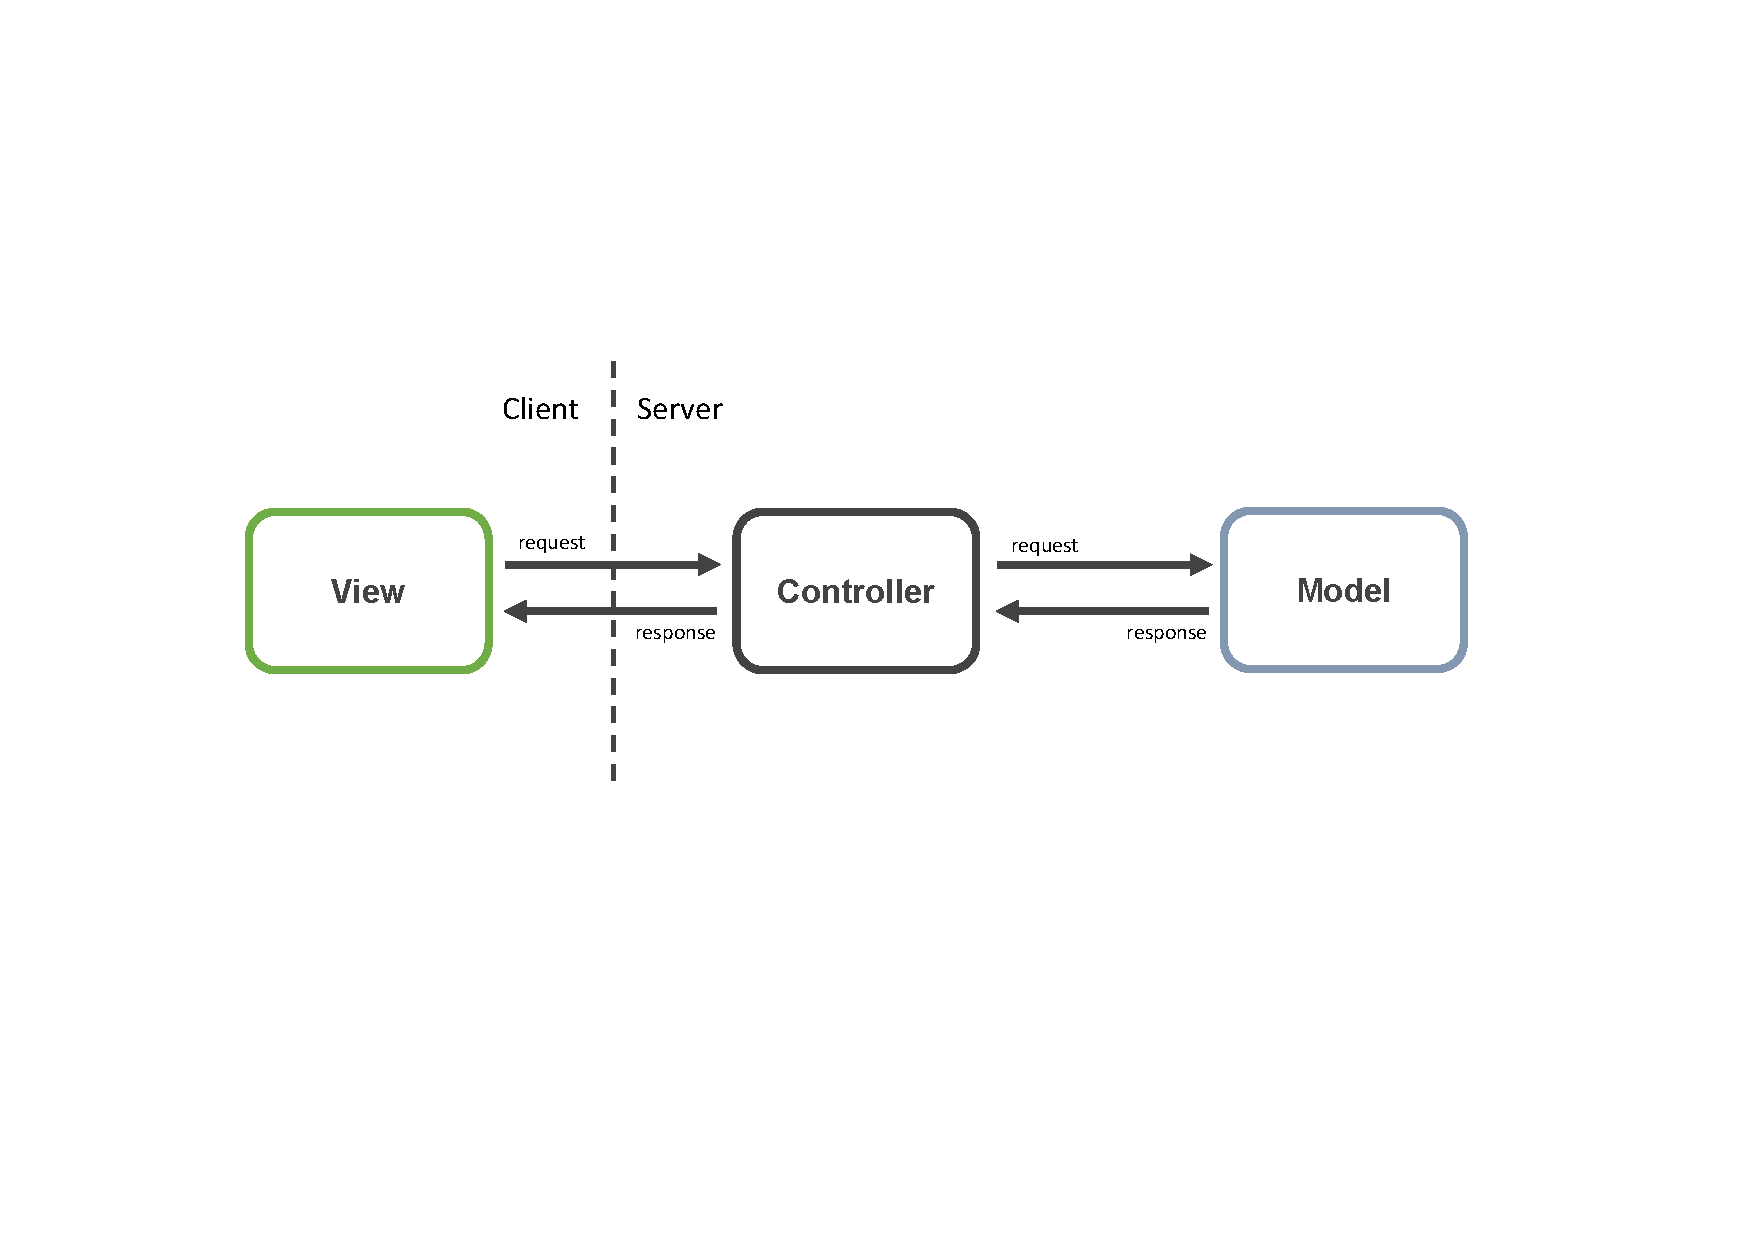
\includegraphics[scale=.7, trim= 4cm 7cm 3cm 5cm, clip]{004serversidemvc.pdf}
  \caption{MVC in a server-client environment \cite[as in][]{ChristianAlfoni.2015}}
  \label{fig:serversidemvc}
\end{figure}

\section{Comparison of the software patterns}

In this section, the Flux and the MVC pattern will be compared. Now that the reader has a basic understanding of what the Flux pattern is about and what it will be compared to it is easier to develop an opinion based on the provided facts. When new software patterns are introduced, it is essential to carefully and critically compare them to existing ones and evaluate their usefulness in the modern software environment, where they can possibly be used.

\subsection{General facts and misconceptions}

% write about data only being updated over the controller is sometimes a big overhead
% maybe include wrong graphs?
% react does not really have a model itself

When casually searching the Internet for the Model View Controller pattern, many visual representations of the software architecture can be found. In many cases the diagrams show the MVC-triad with arrows in facing different directions, unidirectional and bidirectional, leading to confusion and raising the question in what direction data flows exactly. 

Diagrams that show the Model update the View and the View in return update the Model stimulated by user input are quite simply wrong. This is a common misconception. Change of the application state should only be triggered over the Controller. Everything else would imply a violation of the MVC pattern.

In this bachelor's thesis there are two representations of MVC (\ref{fig:tradmvc} and \ref{fig:fowlermvc}). Both representations show the same components but different relations. It must be understood though, that data-flow still goes in one direction. Different names for relations may switch the directions of some arrows in a diagram but do not change the semantic meaning of the MVC pattern.

In the presentation where Facebook introduces the supposedly new software architecture Flux (\cite{youtube.2014}), the speaker presents the audience a visualization of MVC that can be seen in the Figure \ref{fig:mvcalafacebook}. Facebook talks about how complicated the debugging process was because of countless bidirectional relations between the View and the Model components. To the attentive reader it should be clear, that a bidirectional relation between the View and Model component regarding to data-flow implies a violation of the MVC pattern. The question arises if Facebook's engineers had understood the programming paradigm MVC before developing an allegedly new programming paradigm?

% way react works view easily can update model

\begin{figure}
  \centering
  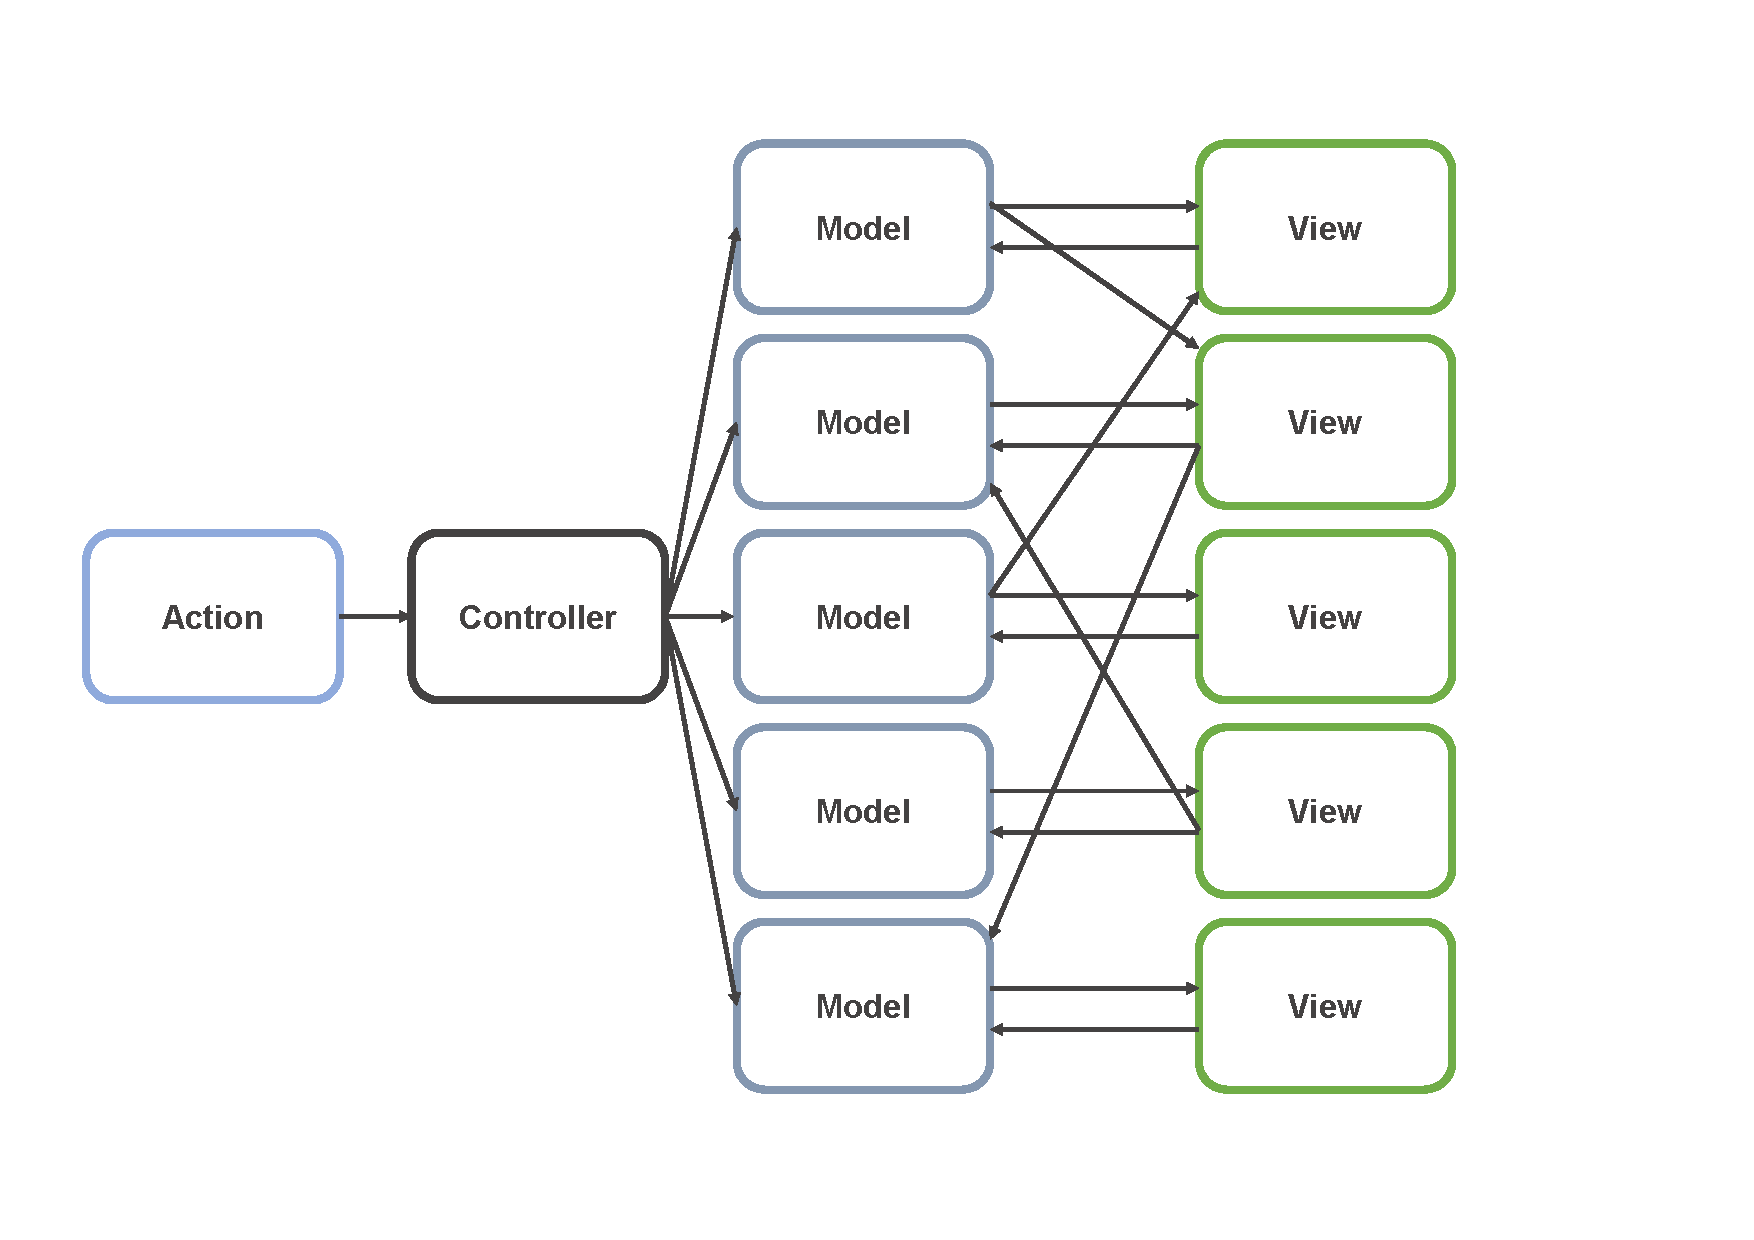
\includegraphics[scale=.6, trim= 1cm 2cm 0 2cm, clip]{003MVCalafacebook.pdf}
  \caption{MVC as Facebook describes it in \cite[11:10]{youtube.2014}}
  \label{fig:mvcalafacebook}
\end{figure}

\subsection{Similarities of Flux and MVC}

Looking at the illustrations of Flux (\ref{fig:FluxArchitecture}) and MVC (\ref{fig:tradmvc}) it can be observed that there are similarities. Flux achieves its unidirectional data-flow by only changing the Store's data by dispatching an Action containing relevant user input data over the Dispatcher. Comparing this behavior to the MVC application architecture, it should be clear that the operation of a change in the Model triggered by a user stimulus handled by the Controller is a quite similar behavior.

One of Flux's biggest advantages, according to Facebook, is the possibility of having global Stores. These global Stores can be used for an application state which has to be used in many different parts of the application e.g. a notification counter that shows the user a count of unread messages. Traditional MVC according to Fowler (\cite[\#ModelViewContoller]{MartinFowler.2006}) needs to have a Controller-View pair for every screen in the user interface but also one global Model that stores the application's state. In most cases though, it is recommended to also divide the Models into the logic sections of the application to make the code more transparent and easier to read and debug. This is very similar to how Flux handles global data. Like in Flux in MVC it is also allowed for more Views to observe the same model.

The MVC triad consists of three components: the View, the Model, and the Controller (\ref{fig:tradmvc}, \ref{fig:fowlermvc}). One could add the User as the fourth optional component that makes the architecture easier to understand. It is the user's stimulus that triggers every action or state change in the application. When looking at the Flux pattern (Figure \ref{fig:FluxArchitecture}) there are also three components that have the same function as the corresponding components in the MVC diagram. Flux's Dispatcher, for instance, could be seen as MVC's controller and the Store is similar if not identical to MVC's Model.

% compare mvc to flux and see the similarities. even tough the patterns are similar it is a good pattern though. Real advantage is immutability though, talk about this later maybe?
% store is global, mvc has no best practice... maybe singleton

\subsection{Differences of Flux and MVC}

One of the biggest differences between Flux and MVC is the way the View component reacts to a change in the application state. In the Flux pattern the View is updated by injecting the new application state into the View. The View component is a strict representation of what has to be displayed at a certain state. Updates therefore happen implicitly. MVC on the other hand handles updates in the application state by binding the View to certain values and thus observing the Model. When a Controller modifies the Model every View that has bound its view-components on data in the Model can automatically update. The MVC View updates itself automatically whereas Flux's View component is updated by the new state that is injected into it.

Another big difference is the way application state is modified. As mentioned before, Flux uses a system where Actions that contain data are dispatched to the Stores which then accordingly react to the dispatched Action and update their data via reducing functions. MVC on the other hand should not have any logic in its Model. Because the Model should only be a representation of Data the Controller must handle API-calls and directly access the Model to change its data.

% state that flux implicitely updates the view and mvc uses an observer pattern
% stores selectively react to action? MVC?

\subsection{Advantages and Disadvantages of Flux and MVC}

A few years ago web developers could not think about another way to engineer a web application other than sending a fully rendered application View to the client and handling user input logic and state on the server. Programmers therefore can only update the View by triggering a change in the state by executing logic in the corresponding Controller. The biggest problem with this approach is that it violates the constraints of traditional MVC as it was designed initially. The Controller and Model instances only live during an HTTP-request, making it impossible to follow MVC's constraint of persisting a Model state during the lifetime of the application. Another big disadvantage is the fact that the View cannot be automatically updated, nor can it observe the model state because of the additional stateless HTTP-layer.

A disadvantage of both patterns is of course programming overhead. Applying a highly complicated application architecture to software always implies increased programming time. What really matters are the long term advantages tough. By using either the Flux or the MVC pattern when developing web applications it makes components interchangeable and increases the application's scalability. Even web applications written in JavaScript for example can heavily benefit from using either one of the mentioned programming paradigms.

% application model domain model difference -> bragge 19
% serverside cant use persisting global state

\section{Conclusion}

Even though the Flux application architecture seems to be extremely similar to traditional MVC, Flux is still an excellent choice for a web application architecture. On its own, MVC has proven itself over the course of the time of its existence. There has been a big shift in how web applications are build until now. Nowadays, many big web applications are built as single-paged applications and the number is steadily growing. The biggest advantage of having an autonomous application that is executed only on the client opens up the possibility to keep application state on the client without having to reload the web page every single time when the application state changes.

The use of single-page applications do not only enable Flux application architecture to be used, the MVC programming pattern can be applied as well of course. Other frameworks like AngularJS for instance use a special variation of MVC called Model-View-ViewModel (MVVM). It is safe to say that using a programming paradigm like Flux or MVC is of utter importance nowadays when building web applications. Not only does it add structure to the code base, but it also makes code much more readable and easier to understand for developers who have not implemented the application but later have to maintain it.

Initially Facebook presented Flux as a big way forward but upon further review it appears as if Flux was just another variation of MVC. There are many similarities that make the two patterns seem to be very alike. It is honestly disappointing to discover that a much praised and hyped application architecture proposal, which had promised many improvements on how to improve web application development, is just a shallow copy of a present paradigm (MVC) that has existed for many years until now. 

It must be emphasized though that Flux is not a bad application architecture approach at all. All the similarities to MVC make Flux a solid pattern that has its merits on its own. After much research it is clear that both patterns can yield enormous advantages if they are used to design web applications. Having no application architecture at all is of course the worst decision a programmer could make. Also, MVC and Flux seem to be very popular among the web developer community.

Upon further reflection it seems as if Facebook did not research properly and implemented MVC wrong. That was the reason why the company came up with a proposal of an allegedly new paradigm. Proof for this theory is the diagram (Figure \ref{fig:mvcalafacebook}) in the video presentation \cite{youtube.2014} which clearly shows that the gist of the MVC paradigm was not understood correctly. 

After having used Flux as a paradigm for a web application it is clear that the architecture seems to be tailored for one specific framework which is ReactJS. The next chapter will show exactly how Flux perfectly fits into the mindset of ReactJS and how it works really well with the framework making it a very satisfying experience to build an application with a good architecture and seeing the benefits of using such a paradigm.

In conclusion it is very important for web application development to use some form of sophisticated application architecture. The number of applications that rely on some form of web technology is increasing heavily nowadays and thus it is even more important to emphasize the necessity to use a well thought through application architecture.

% initially facebook presented flux as a big way forward
% flux was presented ad
% upon review, after research was completed
% after a closer inspection
% after considering the findings / data
% it is clear -> instead of i believe -> flux has only minor advantages / it is only marginally different
% the advantages to not outweigh / the advantages are negligent in comparison
% after review it was conluded / found --> take it for I
% conclusion facebook lied -> make point upon further reflectoin i came to realize flux not that advantageous as i initially thought
